\lstdefinestyle{mystyle}{
    backgroundcolor=\color{myyellow},
    basicstyle=\ttfamily\small,
    breaklines=true,
    frame=single,
    language=XML
}

\chapter{State-of-the-Art Analysis} \label{ch:state-of-the-ArtAnalysis}
The following chapter constitutes an in-depth exploration of current technologies and methodologies within the automotive industry, with a specific focus on the complexity of vehicular software development. Firstly, the current automotive landscape will be examined, providing a detailed insight into challenges associated with software development in vehicles.

Subsequently, through meticulous analysis of scientific publications, technical reports, and practical implementations, the chapter delves into the radical transformation of the automotive sector facilitated by the concept of Software Defined Vehicle (SDV). This technology, crucial for technological progress and vehicular safety, will be explored from various perspectives. Particularly, the synergy between Cloud, software, and hardware will be investigated, highlighting solutions proposed by major industry players and analyzing their applications, benefits, and limitations.

The objective is to offer a comprehensive overview of current dynamics, emphasizing the pivotal role of SDV in the evolution of the automotive industry.

\section{Current Automotive Software Development}

In the past, the automotive industry advanced primarily through the development of technologies in mechanical engineering, focusing on perfecting combustion engines. Nowadays, the paradigm has radically changed due to multiple factors, including electrification, automation, shared mobility, and connected mobility.

Software technology development in the automotive field can be metaphorically compared to what has happened in smartphone development, as highlighted in the manifesto document regarding Bosch's Software Defined Vehicle (SDV) \cite{SDVBoschMobility}.

The ultimate goal is to achieve simple and user-friendly devices that fully meet the user's needs. Currently, many customers express dissatisfaction because their cars do not offer the same functionality and ease of use common in smartphones. Many ask: Why can't my \$50,000 car perform the same tasks as my \$300 smartphone?

A key difference between the automotive and smartphone industries is the level of complexity, which brings with it a number of issues.

\subsection{difficulties}
We can analyse in depth the problems of the current automotive software that is being developed via 4 main difficulties:

\begin{itemize}
    \item Specialized Hardware: Today's vehicles are still complex systems of systems. Each subsystem in a car, from brakes to transmission, is a complex entity, supplied by a different manufacturer and integrated with a unique software architecture. The level of complexity and the need for seamless interoperability between systems far exceeds that of today's smartphones.
    \item Time: The software production pipeline involves many development and testing steps with a not inconsiderable amount of time spent on each one. This is greatly increased by the presence of different components, so development time must be considered for each different unit of the system.
    \item Cost: The complexity of the software systems in vehicles entails very high costs, aggravated by the fact that the test phase is often carried out directly on the boards (for hardware requirements), which means a much longer production process, especially in the event of errors.
    
    \begin{figure}[h]  % 'h' significa che la figura viene posizionata qui
        \centering
        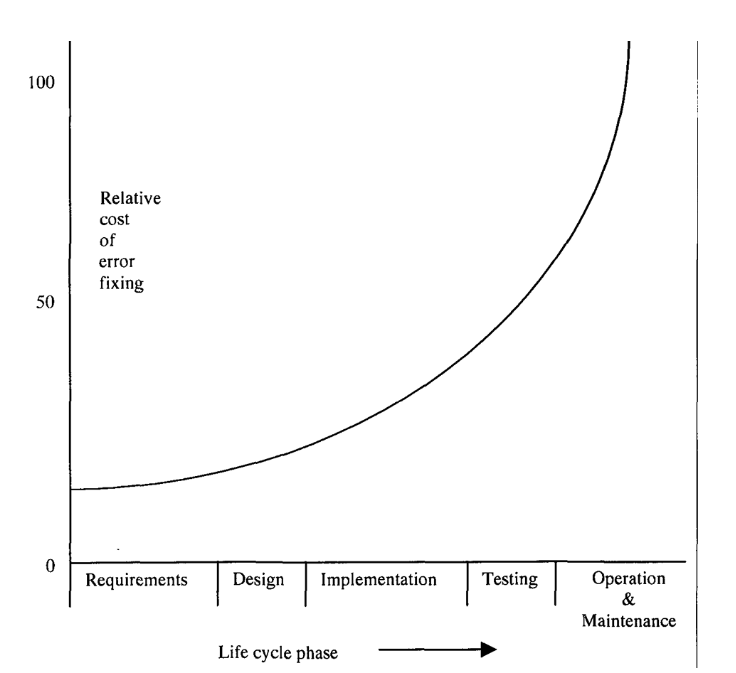
\includegraphics[width=0.9\textwidth]{images/costs_of_errors_correction_in_software_development.png}  % Sostituisci 'nome_immagine' con il nome del tuo file immagine e l'estensione
        \caption{Cost of fixing errors increases in later phases of the life cycle \cite{CostsOfSoftwareDeveloping}}
        \label{fig:WorldAutomobileProduction}
      \end{figure}

    \item Human Safety Security: Automotive embedded software must meet stringent reliability and security requirements, while delivering performance and a reasonable memory footprint. To develop automotive embedded software, you need the right tools that meet safety and security standards to evaluate, prototype and test your software.
\end{itemize}

What lessons can be drawn from the study of barriers that can be applied to the vehicle lifecycle? Historically, the vehicle lifecycle has been characterised by the simultaneous production and deployment of tightly integrated hardware and software. Once the vehicle was in the hands of the consumer, its characteristics remained largely unchanged until the end of its life. However, the SDV paradigm introduces the possibility of decoupling hardware and software release dates, a prerequisite for adopting a digital-first approach. This approach brings the design and virtual validation of the digital vehicle experience to the forefront of the lifecycle.
It also requires the application of the digital-first concept, which means that new ideas for the vehicle experience are first explored in virtual environments to ensure early user feedback, long before any custom hardware needs to be developed or a physical test vehicle is available. Digital first is the application of design thinking and lean startup principles, originally rooted in internet culture, to the tangible realm of automotive development.

%“Automakers and their suppliers need to continuously review and improve the testing approach in design and development, as well as look for new tools that automate and increase test coverage of their products,” Giallorenzo explained. “Cloud emulation is a major innovation that is coming to the industry to facilitate development and testing. Historically, testing of embedded software solutions has been hindered by the lack of chipsets and hardware, which is required to properly test complete hardware-plus-software solutions. This was particularly painful during the recent COVID-induced supply chain crunch."

\section{Introduction to Software Defined Vehicle}
The Software Defined Vehicle represents the new frontier of automotive manufacturing and is poised to completely change the paradigm of automotive production. 

If we imagine bringing a feature update to one of today's vehicles, it will most likely take anywhere from one to seven years from the idea to when that feature is actually perceptible in the production vehicle; this takes so long because the vehicles produced up to this point have not been designed with frequent updates in mind \cite{SDVBosch}.
Traditionally focused on physical functionality, the automotive industry has evolved from early electronic features such as airbags, vehicle stabilisation and braking systems to modern driver assistance and even automated driving. 
The current shift towards a digital experience is possible thanks to vehicle design that includes software integration as a fundamental part. Software should no longer be seen as an accessory to the vehicle, but as an integral part of the vehicle itself.

The simultaneous efforts of major automotive companies such as Bosch, Renault and Stellantis, in collaboration with leading computer developers such as Arm, BlackBerry and AWS, have given rise to the Software Defined Vehicle concept, which they define as "any vehicle that manages its own operations, adds functionality and enables new features primarily or entirely through software" \cite{blackberrySDV}.

It is evident that the Software Defined Vehicle represents the future of the automotive industry, promising an enriched and enduring user experience, coupled with the evolution of automotive technologies. This section further elucidates the current state of the industry, highlighting the key players that are working in the industry as a enablers to develop the SDV technologies, and  the benefits of this innovation.

\subsection{Enablers}
The software defined vehicle solution is nowadays being considered by several companies as the manifesto of a new era of vehicle development. An example is given by the renault group, which in an overview of its products describes: "Today, it is already possible to make remote updates of some vehicles via the Firmware Over The Air (FOTA) system. This keeps the vehicle safe by making it easier and faster to improve the on-board system and apply patches. Tomorrow, the Software Defined Vehicle's flexible and scalable architecture will enable the faster development and integration of new features throughout the vehicle lifecycle, directly into the cloud, that is, in secure online servers accessible from anywhere and anytime" \cite{SDVRenault}. 

Two key technology players, Arm and AWS, have played a pivotal role in advancing SDV by working together to define standards that accelerate technology development.
\begin{itemize}
    \item Arm, a leading semiconductor design and software company, is a pillar in the advancement of SDV technology. Focusing on the development of energy-efficient processors and technologies, Arm's contributions enable SDVs to efficiently manage their operations, add functionality and introduce new features through the development of general-purpose processors that can be used in the cloud for software development and maintenance, and in the vehicle itself to maintain computing continuity.
    \item Amazon Web Services (AWS), a global leader in cloud computing, offers scalable and secure solutions for real-time application updates, enhanced connectivity, and efficient data management. The AWS services and technologies will be in depth described in the futher chapters.
\end{itemize}

The collaborative efforts of this two companies contribute to shaping a future where vehicles are not only defined by their physical attributes but are also dynamic entities capable of continual software-driven enhancements and innovations.

\subsection{Benefits}
